\chapter{Kiến trúc tổng quan của hệ thống}
\section{Giới thiệu}
\begin{figure}[ht]
\begin{center}
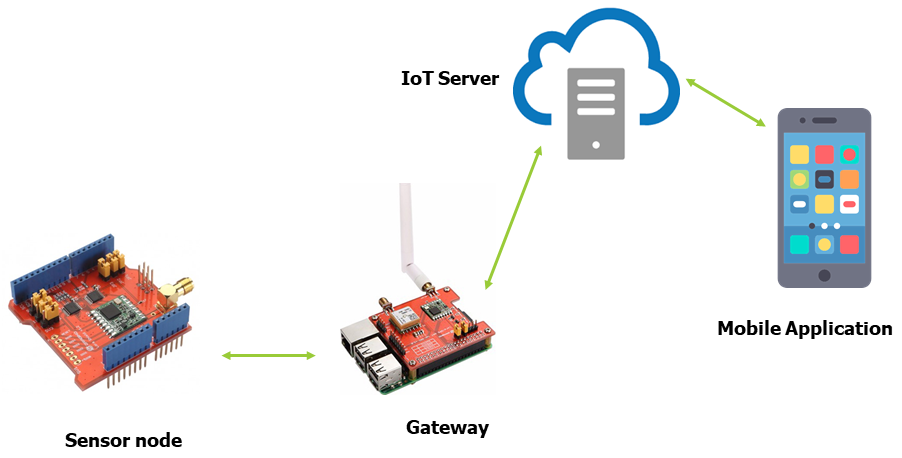
\includegraphics[scale=0.6]{image2/gioi-thieu-chuong-2.png}
\end{center}
\caption{Kiến trúc tổng quan hệ thống}
\end{figure}
Hệ thống Lora được sử dụng trong IOT vì LoRa có thể được áp dụng rộng rãi trong các ứng dụng thu thập dữ liệu như sensor network trong đó các sensor node có thể gửi giá trị đo đạc về trung tâm cách xa hàng km và có thể hoạt động với battery trong thời gian dài trước khi cần thay pin .Một đặc thù riêng biệt, ở môi trường nông nghiệp thì việc truyền dữ liệu từ các cảm biến và trung tâm, và từ trung tâm tới các thiết bị chấp hành sẽ gặp phải các khó khăn về khoảng cách, dễ bị tác động của môi trường,...dẫn đến hệ thống không hoạt động ổn định. Ngoài Zigbee, LoRa là một lựa chọn tuyệt vời. 
Về tổng quan hệ thống bao gồm:
\begin{enumerate}
    \item Các sensor node bao gồm 1 board lora và 1 board arduino. Các node này có nhiệm vụ truyền nhận dữ liệu trong mạng. Giúp dữ liệu từ các cảm biếm có thể đến gateway.
    \item Gateway bao gồm 1 Lora và 1 raspbery. với khả năng tính toán của raspberry thì sẽ đẩy được nhiều dữ liệu lên server cùng một lúc.
    \item Server trức mắt sử dung mqtt.MQTT (Message Queuing Telemetry Transport) là một giao thức gởi dạng publish/subscribe sử dụng cho các thiết bị Internet of Things với băng thông thấp, độ tin cậy cao và khả năng được sử dụng trong mạng lưới không ổn định.

    Bởi vì giao thức này sử dụng băng thông thấp trong môi trường có độ trễ cao nên nó là một giao thức lý tưởng cho các ứng dụng M2M.
    
    \item Application là điện thoại hoặc PC. Giúp người dùng theo dõi dữ liệu trong hệ thống mạng.
\end{enumerate}

\section{Kiến trúc hệ thống}
Hệ thống bao gồm các gateway được đặt ở những nơi có điện và có khả năng kết nối internet. Vì gateway tiếp nhận nhiều dữ liệu nên tiêu tốn nhiều điện cần đặt ở nơi có nguồn điện ổn định.Internet để kết nối lên server.\\
Gateway sẽ kết nối dữ liệu với các node xung quanh để truyền dữ liệu, cấp ID, giúp tìm đường truyền...Các node sẽ thực hiện kết nối với các node xung quanh sao cho dữ liệu truyền đi là tốt nhất.
\newpage
\begin{figure}[ht]
\begin{center}
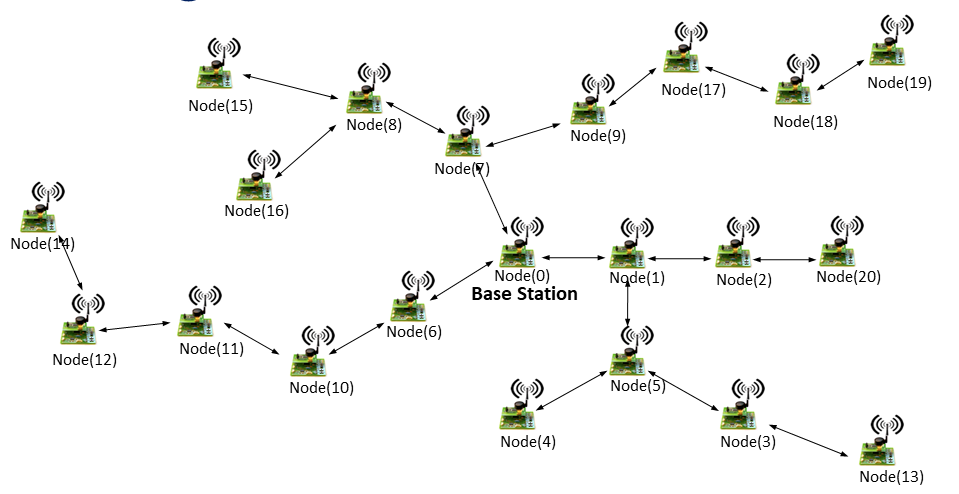
\includegraphics[scale=0.6]{image2/kien-truc-he-thong.png}
\end{center}
\caption{Kiến trúc hệ thống}
\end{figure}

\section{Kiến trúc node cảm biến}

\begin{center}
    \begin{figure}[htp]
    \begin{center}
     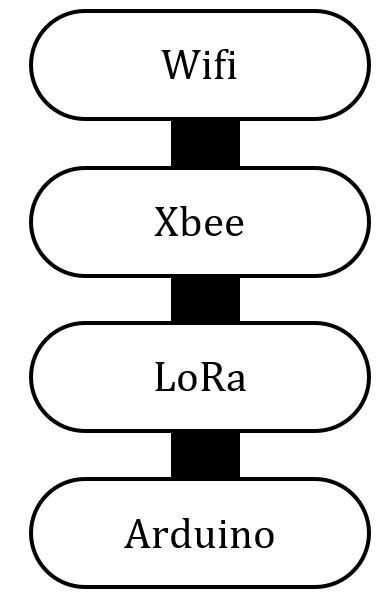
\includegraphics[scale=0.4]{image2/node.JPG}
    \end{center}
    \caption{Kết nối với node cảm biến.}
    \end{figure}
\end{center}

Bao gồm 4 module chính:
\begin{itemize}
    \item Wifi - module giao tiếp không dây, sử dụng mạng wifi. Dùng để cập nhật firmware cho các node cảm biến.
    \item Xbee - module giao tiếp không dây, sử dụng tín hiệu radio có tần sóng ngắn. Dùng để cập nhật firmware cho các node cảm biến.
    \item LoRa - module giao tiếp không dây, sử dụng tín hiệu sóng vô tuyến (radio) với dải băng tần không được cấp phép (433MHz). Dùng để gửi dữ liệu từ các node cảm biến đo đạc được bằng các sensor được gắn trên đó.
    \item Raspberry Pi 3 - Android Things, điều khiển các hoạt động của LoRa (gửi/nhận dữ liệu, quản lý các node cảm biến trong mạng lưới). Đồng thời xử lý dữ liệu nhận được theo chuẩn đã quy định trước khi đưa tất cả dữ liệu lên server.
\end{itemize}

\section{Kiến trúc node gateway}

\begin{center}
    \begin{figure}[htp]
    \begin{center}
     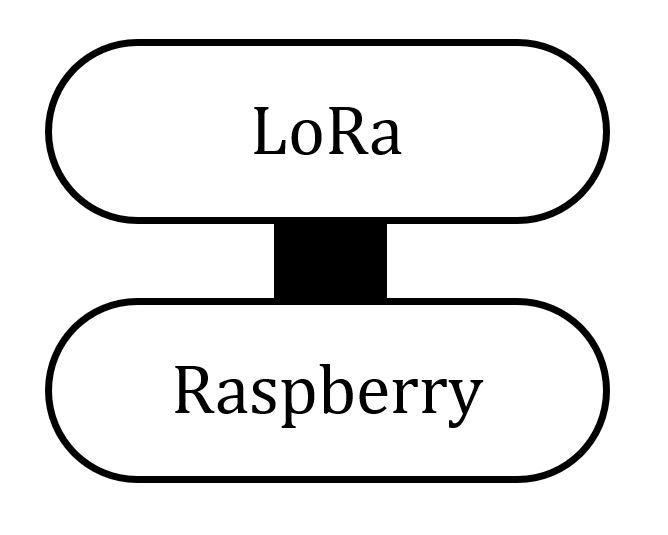
\includegraphics[scale=0.3]{image2/gateway.JPG}
    \end{center}
    \caption{Kết nối với node gateway.}
    \end{figure}
\end{center}

Bao gồm 2 module chính:
\begin{itemize}
    \item LoRa - module giao tiếp không dây, sử dụng tín hiệu sóng vô tuyến (radio) với dải băng tần không được cấp phép (433MHz). Dùng để thu thập dữ liệu từ các node cảm biến đo đạc được bằng các sensor được gắn trên đó.
    \item Raspberry Pi 3 - Android Things, điều khiển các hoạt động của LoRa (gửi/nhận dữ liệu, quản lý các node cảm biến trong mạng lưới). Đồng thời xử lý dữ liệu nhận được theo chuẩn đã quy định trước khi đưa tất cả dữ liệu lên server.
\end{itemize}
 
\section{Mô hình giao tiếp không dây}
\subsection{Giao tiếp ở gateway}
\begin{enumerate}
    \item Ban đầu, Gateway sẽ kết nối với tât cả các node có cường độ tín hiệu thu(RSSI) lớn hơn -70dbm.
\begin{center}
    \begin{figure}[htp]
    \begin{center}
     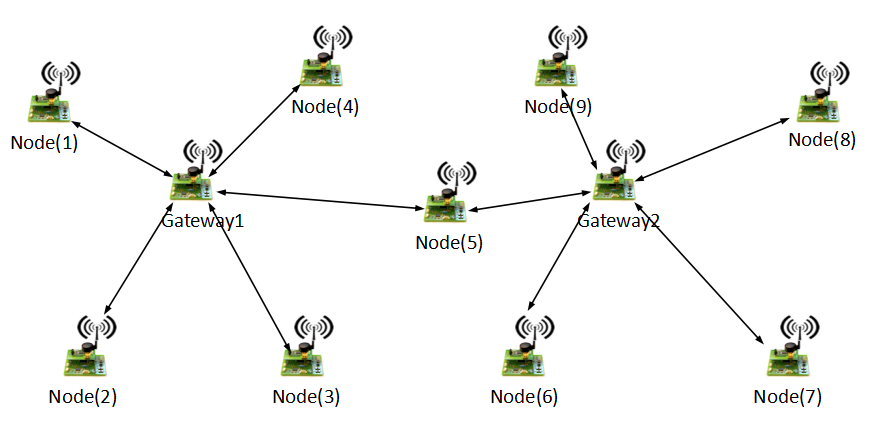
\includegraphics[scale=0.45]{image2/bandau.png}
    \end{center}
    \caption{Gateway kết nối với các node ban đầu.}
    \label{refhinh1}
    \end{figure}
\end{center}
    
    \item Giả sử Node có kết nối với 2 Gateway, thì nó sẽ thực hiện kết nối với node có cường độ tín hiệu thu lớn hơn.
\begin{center}
    \begin{figure}[htp]
    \begin{center}
     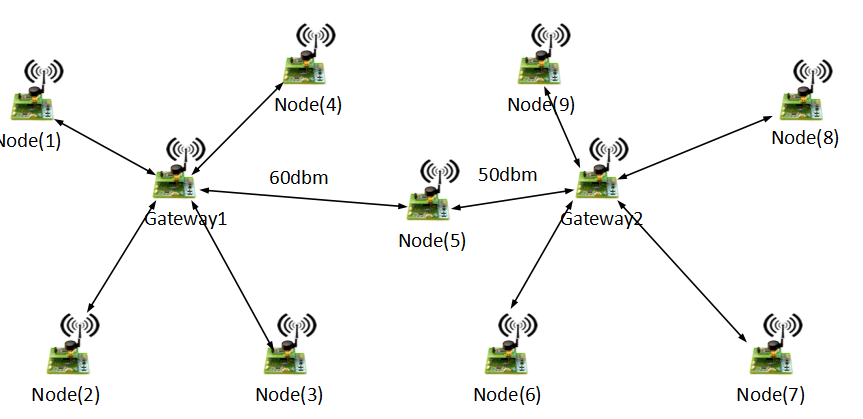
\includegraphics[scale=0.45]{image2/node5.png}
    \end{center}
    \caption{node(5) kết nối với hai Gateway.}
    \label{refhinh1}
    \end{figure}
\end{center}
\newpage
\item với các node ở xa, cường độ tín hiệu thu thấp, nhung không kết nối được với node trung gian nào khác, thì bây giờ thực hiện kết nối với gateway.
\begin{center}
    \begin{figure}[htp]
    \begin{center}
     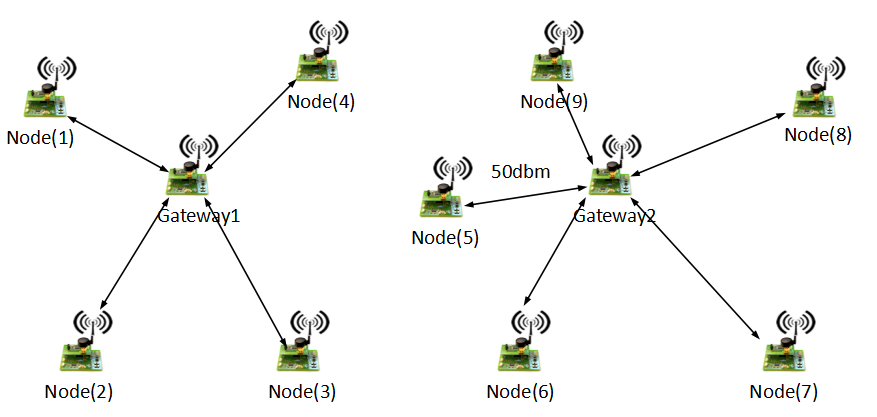
\includegraphics[scale=0.45]{image2/node51.png}
    \end{center}
    \caption{node(5) ngắt kết nối với Gateway1.}
    \label{refhinh1}
    \end{figure}
\end{center}

\item Gateway sẽ cấp địa chỉ IP cho các nối kết nối với nó. Và liên tục cập nhất các node mới, đồng thời kiển tra xem có tất cả có bao nhiêu node kết nối với nó.
\begin{center}
    \begin{figure}[htp]
    \begin{center}
     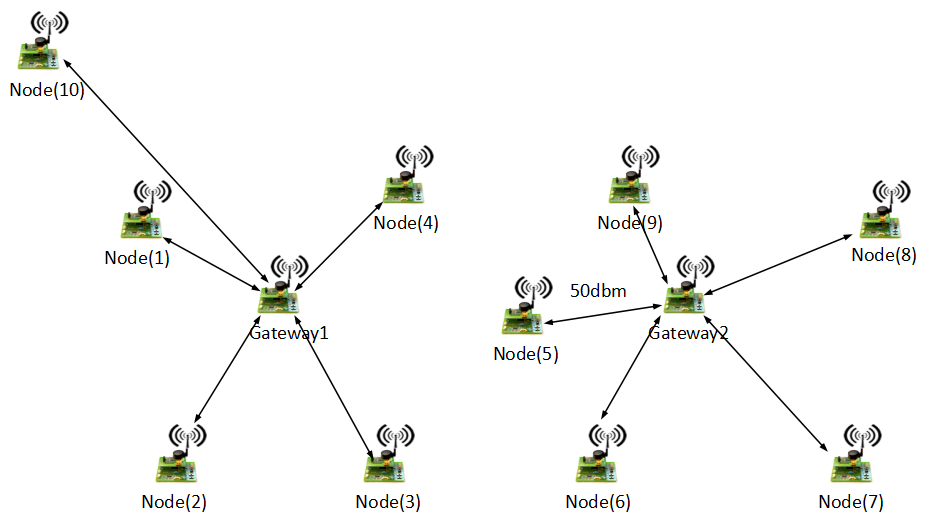
\includegraphics[scale=0.45]{image2/nodexa.png}
    \end{center}
    \caption{các node ở xa kết nối với Gateway.}
    \label{refhinh1}
    \end{figure}
\end{center}
 
    
\end{enumerate}

\subsection{Giao tiếp ở các node}
\begin{enumerate}
    \item các node chưa có kết nối gửi lên Gateway, thì nó sẽ gửi dữ liệu đi đến các node khác, kiển tra xem node đó đã kết nối hay chưa, rồi dựa vào các thông số như cường độ thu tín hiệu, số node trung gian cần phải qua để đến được gateway, số node hiện tại gateway đã kết nối,rồi quyết định kết nối với node phù hợp nhất.

\begin{center}
    \begin{figure}[htp]
    \begin{center}
     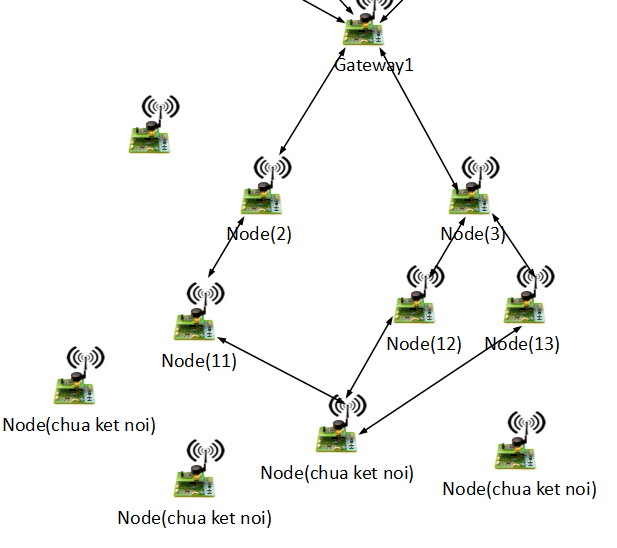
\includegraphics[scale=0.45]{image2/chuaketnoi.png}
    \end{center}
    \caption{Bắt tín hiệu các Gateway bên cạnh.}
    \label{refhinh1}
    \end{figure}
\end{center}

\begin{center}
    \begin{figure}[htp]
    \begin{center}
     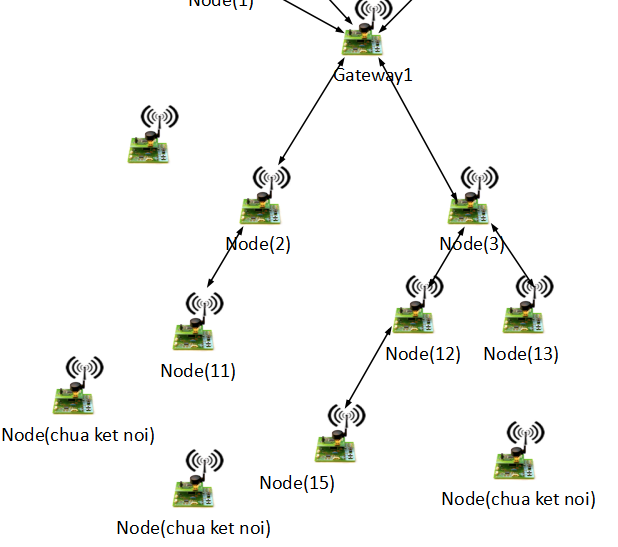
\includegraphics[scale=0.45]{image2/daketnoi.png}
    \end{center}
    \caption{Kết nối với node phù hợp.}
    \label{refhinh1}
    \end{figure}
\end{center}
\end{enumerate}
